\documentclass[11pt,a4paper]{report}

\usepackage{mathtools, amsmath, listings, graphicx, amssymb, nth, multirow, longtable, hyperref, caption}
\usepackage[utf8]{inputenc}
\usepackage[table]{xcolor}

\usepackage[backend=bibtex]{biblatex}
\addbibresource{ref.bib}

\usepackage{geometry}
\geometry{margin=1in}

\makeatletter

% ------------------ <Convenience Commands> --------------------
\graphicspath{ {figures/} }

\newsavebox\myboxA
\newsavebox\myboxB
\newlength\mylenA

\newcommand*\xoverline[2][0.75]{%
    \sbox{\myboxA}{$\m@th#2$}%
    \setbox\myboxB\null% Phantom box
    \ht\myboxB=\ht\myboxA%
    \dp\myboxB=\dp\myboxA%
    \wd\myboxB=#1\wd\myboxA% Scale phantom
    \sbox\myboxB{$\m@th\overline{\copy\myboxB}$}%  Overlined phantom
    \setlength\mylenA{\the\wd\myboxA}%   calc width diff
    \addtolength\mylenA{-\the\wd\myboxB}%
    \ifdim\wd\myboxB<\wd\myboxA%
       \rlap{\hskip 0.5\mylenA\usebox\myboxB}{\usebox\myboxA}%
    \else
        \hskip -0.5\mylenA\rlap{\usebox\myboxA}{\hskip 0.5\mylenA\usebox\myboxB}%
    \fi}
\makeatother

\hypersetup{colorlinks=true, linkcolor=blue}

\DeclarePairedDelimiter\ceil{\lceil}{\rceil}
\DeclarePairedDelimiter\floor{\lfloor}{\rfloor}

\newcommand{\ts}{\textsuperscript}

% ------------------ </Convenience Commands> --------------------

\begin{document}

% ------------------ Title Page --------------------

\begin{titlepage}
	\centering
	
\includegraphics[width=0.15\textwidth]{brandeis-seal}\par\vspace{1cm}
	{\scshape\LARGE Brandeis University \par}
	\vspace{1cm}
	{\scshape\Large Senior Thesis in Computer Science\par}
	\vspace{1.5cm}
	{\huge\bfseries Graph Matching, Pattern Learning,\par and Protein Modeling \par}
	\vspace{2cm}
	{\Large\itshape Wei Qian\par}
	\vfill
	Supervised by\par
	Prof. \textsc{Pengyu Hong}
	\vfill

	{\large \today\par}
\end{titlepage}

% ------------ Table of Contents ----------------

\tableofcontents

% ----------------- Chapters ----------------------

\chapter*{Acknowledgments}

When I asked Professor Storer to supervise me on a thesis on the graph isomorphism problem, he was hesitant.
He only acquiesced when I persuaded him that my future was secure with a fantastic job, and that my primary objective was the pursuit of questions that were of nothing but personal interest to me.
In many respects, his skepticism proved well founded.

This work has been incredibly challenging, both in that the body of existing work on GI is so large, and in that few visible niches of it exist which are promising and not thoroughly explored.
Over the past year I have poured my time and energy into this project, and have found it unbelievably energizing to do so.
I have been thrilled to find interesting properties in problems surrounding GI, and have had an equal number of frustrations in finding that my results had been previously discovered.
Moreover, it has been illuminating to begin to understand a hidden world of graph theory which had before seemed either trivial or intractably complex.

I would like to thank Professor Storer for the initial bout of skepticism about this project, as it shaped this project and experience for the better.
But I would also like to thank him for the amount of advice and freedom that he has supported me with on this project.
It has kept me on track to focus on my real goal for the semester, which was to learn and grow.
I have learned advanced techniques in GPU calculation, proof techniques in abstract algebra, and gotten the chance to reason with established problems in new and interesting ways.
My skill set has been broadened by this project which has deeply challenged me and always kept me on my toes.

I would like to thank my advisors (Prfs. Storer, Di Lillo and Torrey), the Computer Science department, and my friends and family for all of the different kinds of support and encouragement that have brought me to successful completion of this project.

\chapter*{Abstract}

Given a graph, count the number of closed walks (called cycles) of every length that pass through each vertex in the graph.
Counting the number of cycles gives us a vector which describes a kind of local resonance, a description of the localized area around each vertex within the graph.
This idea is a numerical property, called an invariant, which is highly information dense--able to detect differences between graphs (or vertices) with high probability, but not sufficient to verify that two graphs (or vertices in a single graph) are the same.
It turns out that we can calculate the number of Cycles very quickly, relative to how much information it gives us.

The number of graphs you can create, even over a small number of vertices, is very large.
However, the number is \emph{much} larger if you consider different labelings of the same graph to be distinct.
This difference matters in many contexts, but is made clear through examining standard random graph generators, which treat different labelings of the same graph as if they are different graphs. 
This is not a problem in and of itself (it makes sense in many practical contexts), but it warps theoretic arguments about the runtime of algorithms over `random' graphs, in ways that we can describe through probability, algebraic proof and experimental results.
It turns out that making up our own random graph generators can actually improve upon this state of affairs in a quantifiable way.

\chapter*{An Open Source Project}

An interesting aspect of this thesis has been that I have placed every incremental iteration of my work online, through the git version control system and GitHub.
Every element, from my reading notes, to my mid-semester reports, to my code, results, and datasets: everything has been kept in a central repository, and every change has been committed and logged.
Alongside this choice, I have decided that every line of code I have written is open source and publicly available for use; licensed under the Creative Commons Attribution-ShareAlike 4.0 International License.

There are three reasons to make this thesis as an open source, version controlled work.
\begin{enumerate}
\item{
Research in academia is far too often done in the dark, and only once the conclusion has been drawn and sufficiently polished does the general public get to learn about it. 
This falsely represents scientific inquiry as a lightning bolt, a blinding and stark progression from correct idea to correct idea. 

In reality we all explore ideas that fail, we all have intuitions that turn out to be incorrect.
The reality of research is much more one of lightning's infinitesimally branching electrical charges (with eventual connection and brilliance). Though this report presents a well coordinated and rehearse set of conclusions, this is not a reflection of all of the work that was done. The GitHub source provides the other pieces of this puzzle.
}
\item{I work on a personal laptop, a school desktop, and occasionally a public workstation. Transferring data (of all sorts) between these computers is tiresome and error prone without a VCS.}
\item{Everyone does better work when they know that their work could be observed.}
\end{enumerate}

The work is available \href{http://www.github.com/gbdubs/thesis}{on my personal github page}, and will be there for the foreseeable future.

\chapter{Graph Matching}
\label{chap: graphmatching}

\section{Introduction}

In order to extract the common pattern from graphs, we need to first compare two graphs and match\footnotemark the relevant part together to better summarize them. However, since the largest common subgraph problem is NP-complete, the graph matching problem we are dealing with is also NP-complete (even though you can argue it's NP-hard in some other definition). Therefore, we must look for good suboptimal solutions via approximation.
\footnotetext{The graph matching here is different than the "matching" problem in graph theory where the \emph{matching} is a set of pairwise non-adjacent edge.}\\

There are two main approaches for graph matching. One approach involves the construction of a state-space that can be searched via some brach and bound methods. While some heuristic rule can help us reduce the complexity from exponential to polynomial, the polynomial complexity would still have a high complexity. The second approach employs nonlinear optimization methods like relaxation labeling, which do not search based on the state-space and generally have a much lower computational complexity.\\

In the realm of nonlinear optimization methods and similar to relaxation labeling, here we described a graduated assigned approach developed by Gold and Rangarajan in 1996 and the improvement we made on the algorithm in order deal with larger graphs we encounter today 20 years later.

\section{Syntax and Definition}

Here we use a attributed relational graph (ARG) to represent our spatial pattern. An ARG, $G$, is a \emph{directional} graph with labels on its nodes ($\overrightarrow{N_{a}}$ is the label for the $a$th node in the graph) and edges ($\overrightarrow{E_{ab}}$ is the label for the edge from the $a$th node to the $b$th node). \\

Since two graphs might only match partially by their subgraph or might not have match at all, Gold and Rangarajan add a null node, $\phi$, in each ARG.\\

We then can define the node compatibility function($c_N$) and the edge compatibility function($c_E$) to calculate the compatibility, $C$, between the nodes and edges between two ARGs, $G$ and $G'$. Here, $C_{ai}$ is the compatibility between node $\overrightarrow{N_{a}}$ in $G$ and node $\overrightarrow{N_{i}}$ in $G'$, while $C_{abij}$ is the compatibility between edge $\overrightarrow{E_{ab}}$ in $G$ and $\overrightarrow{E_{ij}}$ in $G'$.\\

The match result is defined as a matrix $M$ where $M_{ai}$ is the probability matching the $a$th node in $G$ to the $i$th node in $G'$.

\section{Problem Definition}

We defined the problem of ARG matching in the following manner. Given two ARG, $G$ and $G'$, we want to find the match matrix $M$ such that the following objective function is minimized:

\begin{equation}\label{eq:energy}
E(M)=-\frac{1}{2}\sum_{a=1}^{G}\sum_{i=1}^{G'}\sum_{b=1}^{G}\sum_{j=1}^{G'}M_{ai}M_{bj}C_{abij}-\alpha\sum_{a=1}^{G}\sum_{i=1}^{G'}M_{ai}C_{ai}
\end{equation}
subject to a two way constraints: $\forall a\ne\phi$, $\sum_{i=1}^{G'}M_{ai}=1$ and $\forall i\ne\phi$, $\sum_{i=1}^GM_{ai}=1$:

\begin{figure}[h]
	\centering
	\captionsetup{justification=centering}
	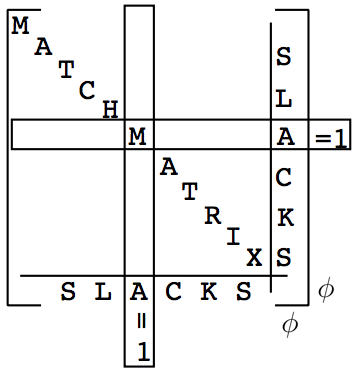
\includegraphics[width=0.25\textwidth]{figs/two_way_constraints.png}
	\caption[Caption for LOF]{\emph{Both rows and columns should sum up to 1 except the row and column involving $\phi$ nodes, which are considered the slack row and slack column.}}
	\label{fig:two_way_constraints}
\end{figure}

\section{Graph Matching by Gold and Rangarajan}

In Gold and Rangarajan's original algorithm, they solve the problem using a graduated assignment method where the two-way constraints are satisfied by normalizing rows and columns iteratively for many rounds (Sinkhorn 1963) and their compatibilities are defined as:
\begin{align} 
& C_{ai}  = \begin{cases}0 & a=\phi \bigcup i=\phi \\c_N(\overrightarrow{N_{a}},\overrightarrow{N_{i}}) & otherwise\end{cases}\\
& C_{abij} = \begin{cases}0 & a=\phi \bigcup b=\phi \bigcup i=\phi \bigcup j=\phi \\c_E(\overrightarrow{E_{ab}},\overrightarrow{E_{ij}}) & otherwise\end{cases} 
\end{align}\\

To expand on their graduated assignment method, we will first need to convert our objective function to an assignment problem. They way we do it is through Taylor series approximation, where given an initial $M^0$, we would have:
\begin{align}
E(M) = & -\frac{1}{2}\sum_{a=1}^{G}\sum_{i=1}^{G'}\sum_{b=1}^{G}\sum_{j=1}^{G'}M_{ai}M_{bj}C_{abij}-\alpha\sum_{a=1}^{G}\sum_{i=1}^{G'}M_{ai}C_{ai}\nonumber\\
= & -\frac{1}{2}\sum_{a=1}^{G}\sum_{i=1}^{G'}\sum_{b=1}^{G}\sum_{j=1}^{G'}M_{ai}^{0}M_{bj}^{0}C_{abij}-\alpha\sum_{a=1}^{G}\sum_{i=1}^{G'}M_{ai}^{0}C_{ai} - Q_{ai}(M_{ai}-M_{ai}^{0})
\end{align}
where
\begin{equation} 
Q_{ai}=-\frac{\partial E}{\partial M_{ai}}\bigg\rvert_{M=M_0}=+\sum_{b=1}^{G}\sum_{j=1}^{G'}M_{bj}^{0}C_{abij}+\alpha C_{ai}
\end{equation}\\

Therefore, minimizing our objective function $E$ based on our Taylor series expansion is equivalent to maximizing 
\begin{equation}
+\sum_{a=1}^{G}\sum_{i=1}^{G'}Q_{ai}M_{ai}
\end{equation}
which is an assignment problem!\\

Therefore, we can run the following algorithm for the graduated assignment:\\
\\
\textbf{Initialize} $\beta$ to $\beta_{0}$, $M_{ai}$ to a random sample from $U(0,1)$\\
\textbf{Begin $A$:} (Do $A$ until $\beta \geq \beta_{f}$)\\
\indent \textbf{Begin $B$:} (Do $B$ until $M$ converges or \# of iterations $>I_0$)\\
\indent $Q_{ai} \leftarrow \sum_{b=1}^{G}\sum_{j=1}^{G'}M_{bj}^{0}C_{abij}+\alpha C_{ai}$\\
\indent $M_{ai}^{0} \leftarrow exp(\beta Q_{qi})$\\
\indent \indent \textbf{Begin $C$:} (Do $C$ until $M$ converges or \# of iterations $>I_1$)\\
\indent \indent  Update $M$ by normalizing across all rows:\\
\indent \indent  $M_{ai}^{1}=\frac{M_{ai}^{0}}{\sum_{i=1}^{G'}M_{ai}^{0}}$ for all $a\neq\phi$\\
\indent \indent  Update $M$ by normalizing across all columns:\\
\indent \indent  $M_{ai}^{0}=\frac{M_{ai}^{1}}{\sum_{a=1}^{G}M_{ai}^{1}}$ for all $i\neq\phi$\\
\indent \indent \textbf{End $C$}\\
\indent \textbf{End $B$}\\
$\beta\leftarrow\beta_{r}\beta$\\
\textbf{End $A$}\\
\textbf{Perform Clean-up Heuristic}\\

Variable and constant definitions can be found as:
\begin{figure}[h]
	\centering
	\captionsetup{justification=centering}
	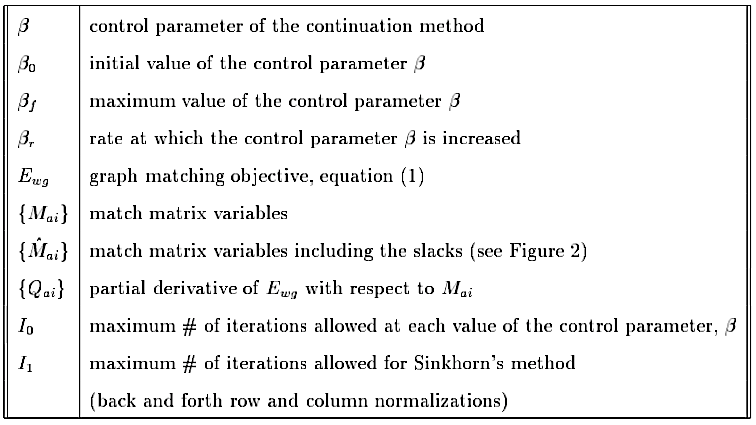
\includegraphics[width=0.95\textwidth]{figs/algorithm_variable.png}
\end{figure}

\section{Implementation Detail}

\subsection{Compatibility}
\label{ssec:compatibility}

To calculate the compatibility, we assume the label/feature follows a Gaussian probability distribution function so that the compatibility function $c_N$ and $c_G$ is defined as:
\begin{equation} 
c_N( \overrightarrow{a}, \overrightarrow{b} )=c_E( \overrightarrow{a}, \overrightarrow{b})=\frac{exp(-\frac{1}{2}(\overrightarrow{a}-\overrightarrow{b})^{T}\Sigma^{-1}(\overrightarrow{a}-\overrightarrow{b})}{(2\pi)^{\zeta/2}|\Sigma|^{1/2}}
\end{equation}
where $\delta$ is the covariance matrix and $\zeta$ is the dimension of $\overrightarrow{a}$ and $\overrightarrow{b}$. Since we assume feature independence, the covariance matrix $\delta$ is the identity matrix, which essentially will give us:
\begin{equation} 
c_N( \overrightarrow{a}, \overrightarrow{b} )=c_E( \overrightarrow{a}, \overrightarrow{b})=\frac{exp(-\frac{1}{2}(\overrightarrow{a}-\overrightarrow{b})^{T}(\overrightarrow{a}-\overrightarrow{b})}{(2\pi)^{\zeta/2}}
\end{equation}

\subsection{Parallel Computing and Caching}

The majority of the computation complexity in the algorithm is in computing the compatibility, especially the edge compatibility.\\

Since the compatibility function defined can be computer independently, one way we could speed up the algorithm is calculating the compatibility in parallel fashion.\\

Another way we could improve the computation time would be through caching, where we can pre compute a node and edge compatibility matrix, as the label is never updated. However, the edge compatibility matrix can be very large and takes a lot of memory to cache, so you might also want to use data structure like \emph{sparse matrix} since the connection matrix (representing edge) is likely to be sparse as well.

\subsection{Heuristic}

In our implementation, we use a very simple heuristic to clean up the match matrix $M$ from a \emph{softassign} matrix to a matrix only with $0$ and $1$. We simply set the largest value (at index $j$) for each row $i$ to 1 and other value to 0. After setting $M_{ij}$ to 1, we also set the entire $j$ column to 0 in order to satisfy the two-way constraints.\\

If you want to be more fancy about this, you can also convert this heuristic problem to a maximum spanning tree problem to make sure all the $M_{ij}$ that you set to 1 have the largest sum.

\subsection{Converge Condition}

In our implementation, we compare the previous match matrix $M^{(0)}$ and the current match matrix $M^{(1)}$, and conclude the matrix converge if the difference is less than some threshold $\iota$:

\begin{equation} 
\sum_{a=1}^{G}\sum_{i=1}^{G'}|M_{ai}^{(0)}-M_{ai}^{(1)}|<\iota
\end{equation}

\subsection{Run Time}
\label{ssec:graphmatchingruntime}

The algorithm takes $\sim15s$ to complete when matching two graphs with $\sim30$ nodes. However, you can certainly adjust the parameter like $I$ and $\beta$ to achieve faster run time.

\section{Testing the Algorithm}
\label{sec:graphmatchingtest}

To test the algorithm, we first set a noise level $\epsilon \in [0,1]$. Then we generate a pattern with $n$ nodes and embed this pattern to $2$ randomly generated graphs, $G$ and $G'$, with $n$ to $n*(1+\epsilon)$ nodes. Once we embed the pattern in these two random graphs, we shuffle the index for each node and add some noise to the node and edge labels:

\begin{equation} 
\overrightarrow{N_{a}} \leftarrow \overrightarrow{N_{a}}  + \chi*\overline{N} \text{ where } \chi \in [0,\epsilon]
\end{equation}
\begin{equation} 
\overrightarrow{E_{ab}} \leftarrow \overrightarrow{E_{ab}}  + \chi*\overline{E} \text{ where } \chi \in [0,\epsilon]
\end{equation}\\

We then run the matching algorithm $match(G,G')$ and get a match matrix $M$. We ignore the match with the null node $\phi$, and calculate the total number of correct match $m$, and the total number of match observed $l$ from the match matrix $M$. Then we can evaluate the performance by $precision$, $recall$ and $F_1 score$:
\begin{align} 
& precision = \frac{m}{l}\\
& recall = \frac{m}{n}\\
& F_1 =2*\frac{precision*recall}{precision+recall}
\end{align}

\section{Improvement and Modification}

While the original algorithm works well with small graphs with 20 to 30 nodes, we run into some problems while matching larger graphs with 50 to 100 nodes and therefore make some improvement to Gold and Rangarajan's original algorithm.

\subsection{Local Minima}

The first problem we encounter is local minima. In this case, the algorithm will generate correct and even perfect match for majority of the test cases. However, for some of the test case, the match result is entirely wrong, which indicates that the graduated assignment process stuck in some local minima.\\

In the original algorithm, if we initialized $M_0$ in the wrong places, the assignment process can easily get stuck in sub-optimal match (local minima). While adjusting $\beta$ and $\beta_r$ can mediate the problem, it does not work well in larger graphs since there are more sub-optimal match. Therefore, we introduce a stochastic process in the algorithm:

\begin{figure}[h]
	\centering
	\captionsetup{justification=centering}
	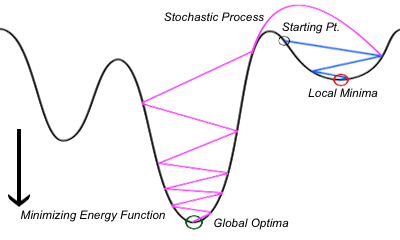
\includegraphics[width=0.46\textwidth]{figs/stochastic.png}
	\caption[Caption for LOF]{\emph{The intuition behind introducing the stochastic process.}}
	\label{fig:stochastic}
\end{figure}

In the stochastic process, we essentially add some small noise to the match matrix at the beginning of step \textbf{$B$}:
\begin{equation} 
M_{ai}^{0} \leftarrow M_{ai}^{0} + \frac{\tau * U(-1,1)}{|G|}
\end{equation}
where $\tau$ is the stochastic/noise level, $|G|$ is the number of node in $G$, and $U(-1,1)$ is a random sample from a uniform distribution between $-1$ and $+1$.\\

Therefore, the updated algorithm becomes:\\
\\
\textbf{Initialize} $\beta$ to $\beta_{0}$, $M_{ai}$ to a random sample from $U(0,1)$\\
\textbf{Begin $A$:} (Do $A$ until $\beta \geq \beta_{f}$)\\
\indent \textbf{Begin $B$:} (Do $B$ until $M$ converges or \# of iterations $>I_0$)\\
\indent \textcolor{red}{$M_{ai}^{0} \leftarrow M_{ai}^{0} + \frac{\tau * U(-1,1)}{|G|}$}\\
\indent $Q_{ai} \leftarrow \sum_{b=1}^{G}\sum_{j=1}^{G'}M_{bj}^{0}C_{abij}+\alpha C_{ai}$\\
\indent $M_{ai}^{0} \leftarrow exp(\beta Q_{qi})$\\
\indent \indent \textbf{Begin $C$:} (Do $C$ until $M$ converges or \# of iterations $>I_1$)\\
\indent \indent  Update $M$ by normalizing across all rows:\\
\indent \indent  $M_{ai}^{1}=\frac{M_{ai}^{0}}{\sum_{i=1}^{G'}M_{ai}^{0}}$ for all $a\neq\phi$\\
\indent \indent  Update $M$ by normalizing across all columns:\\
\indent \indent  $M_{ai}^{0}=\frac{M_{ai}^{1}}{\sum_{a=1}^{G}M_{ai}^{1}}$ for all $i\neq\phi$\\
\indent \indent \textbf{End $C$}\\
\indent \textbf{End $B$}\\
$\beta\leftarrow\beta_{r}\beta$\\
\textbf{End $A$}\\
\textbf{Perform Clean-up Heuristic}\\

Once we incorporate the stochastic process to the algorithm, we gain a significant improvement in $F_1$ score and there is very little chance the match result is entirely wrong:

\begin{figure}[h]
	\centering
	\captionsetup{justification=centering}
	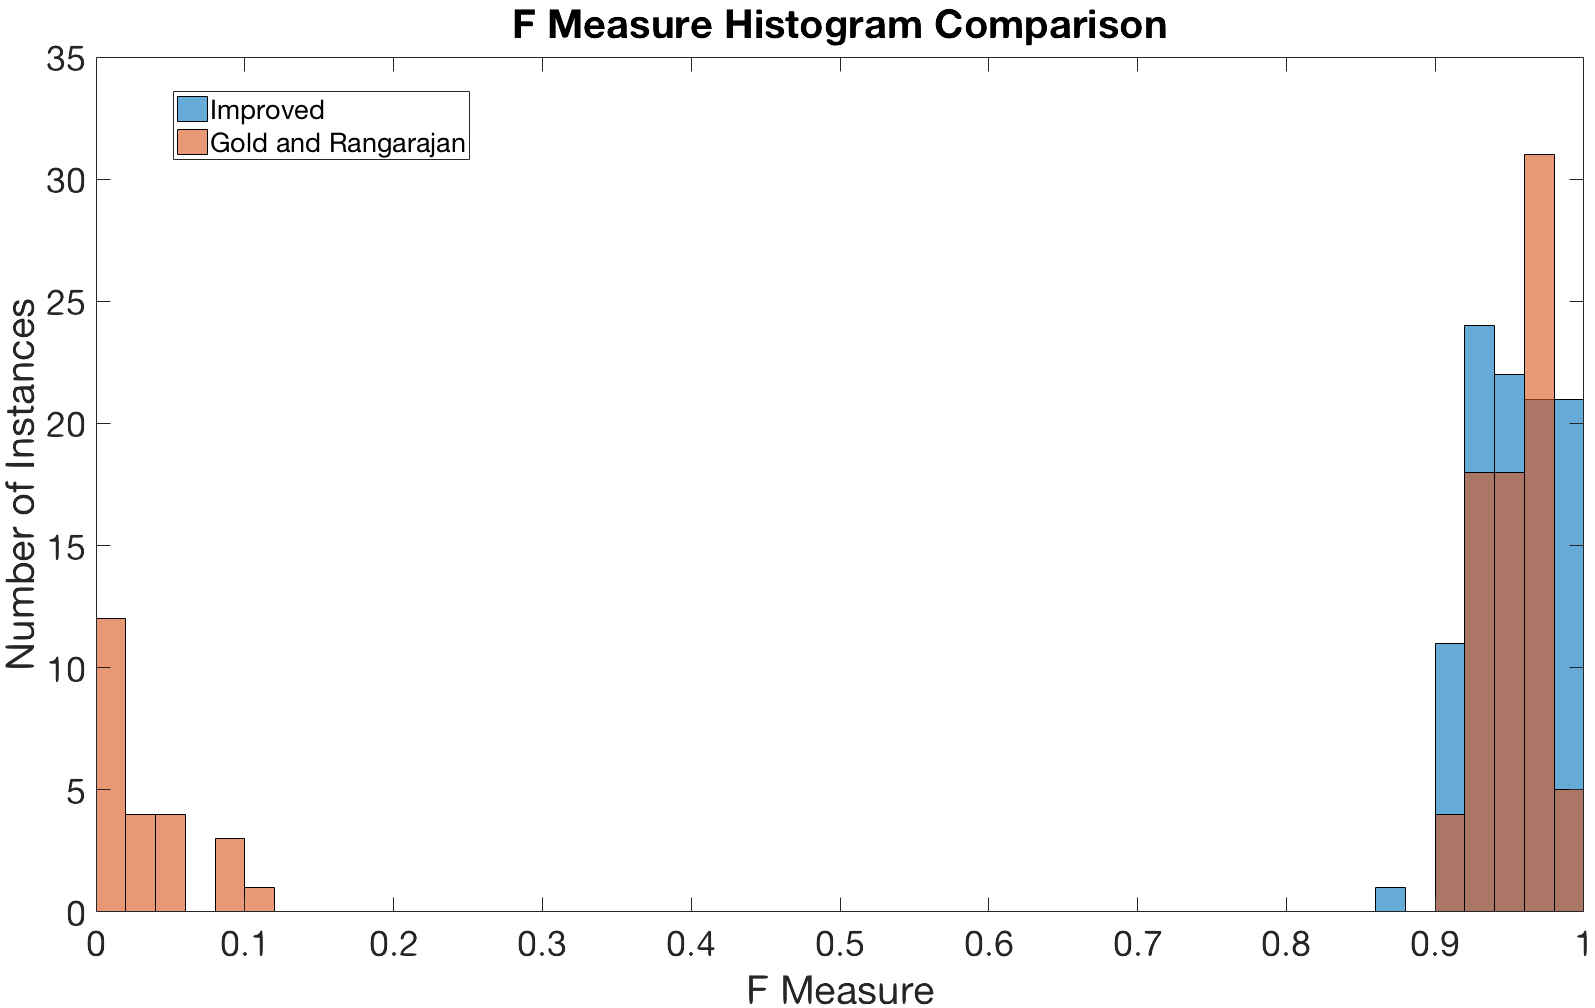
\includegraphics[width=0.85\textwidth]{figs/s_improved.png}
	\caption[Caption for LOF]{\emph{$F_1$ score distribution histogram for the original algorithm (orange) and the improved algorithm with stochastic process (blue).}}
	\label{fig:stochastic}
\end{figure}

\subsection{High Recall + Low Precision}
\label{ssec:nullnode}

The other challenge we encounter is that even though we get high recall rate in a test, we also get low precision rate, which means the algorithm can generate correct match but also force many of the background nodes (i.e. nodes outside of the pattern) matching  to each other.\\

The first explanation came across our mind would be the two test graphs we generated can share pattern outside the embedded one. However, after careful examination, this is proven not the case.\\

Therefore, we examed how Gold and Rangarajan's original algorithm matches background nodes in $G$ to the null node $\phi$ in $G'$. We realized that since the original algorithm define the compatibility function so that any compatibility related to the $\phi$ node will be set to 0. Therefore, the algorithm does not \emph{actively} match background nodes to  $\phi$ node, but \emph{hope} that the background noise does not attract to one specific node, and end up matching with the $\phi$ node.\\

To handle this problem gracefully, we essentially want to create a fully connected null node network that can match to any of the background pattern. Therefore, we rewrite the compatibility function as:

\begin{align} 
& C_{ai}  = \begin{cases}
0 & a,i=\phi \\
c_N(\overrightarrow{N_{a}},\overrightarrow{N_{i}}) & a, i\neq\phi \\
p \text{ percentile of }[C_{1i}, C_{2i},...C_{|G|-1i}] & a=\phi\\
p \text{ percentile of }[C_{a1}, C_{a2},...C_{a|G'|-1}] & i=\phi
\end{cases}\\
& C_{abij} = \begin{cases}
c_E(\overrightarrow{E_{ab}},\overrightarrow{E_{ij}})  & a,b,i,j\neq\phi \\
p \text{ percentile of }\{C_{abij}|a,b,i,j\neq\phi\} & a,b\neq\phi \bigcap i,j=\phi\\
p \text{ percentile of }\{C_{abij}|a,b,i,j\neq\phi\} & a,b=\phi \bigcap i,j\neq\phi\\
0 & otherwise\\
\end{cases}
\end{align}
where $p$ is a percentile we can adjust so that set to 100 to give null node/edge the maximum compatibility every seen while set to 0 to give the minimum compatibility. You can adjust the $p$ to balance the recall and precision rate since higher percentile will encourage nodes match to null node result in low recall but high precision while lower percentile will allow background nodes match together result in high recall but low precision.\\

While this is a lot to unpack, the updated compatibility function essentially create a self-linked edge for null node $\overrightarrow{E_{\phi\phi}}$ and give definition for the compatibility of null node to other real node and self-linked null edge to other edge linking two real nodes. Since we don't normalized the slack row and column (match result for null node), this is equivalent to create a fully connected null node network:

\begin{figure}[h]
	\centering
	\captionsetup{justification=centering}
	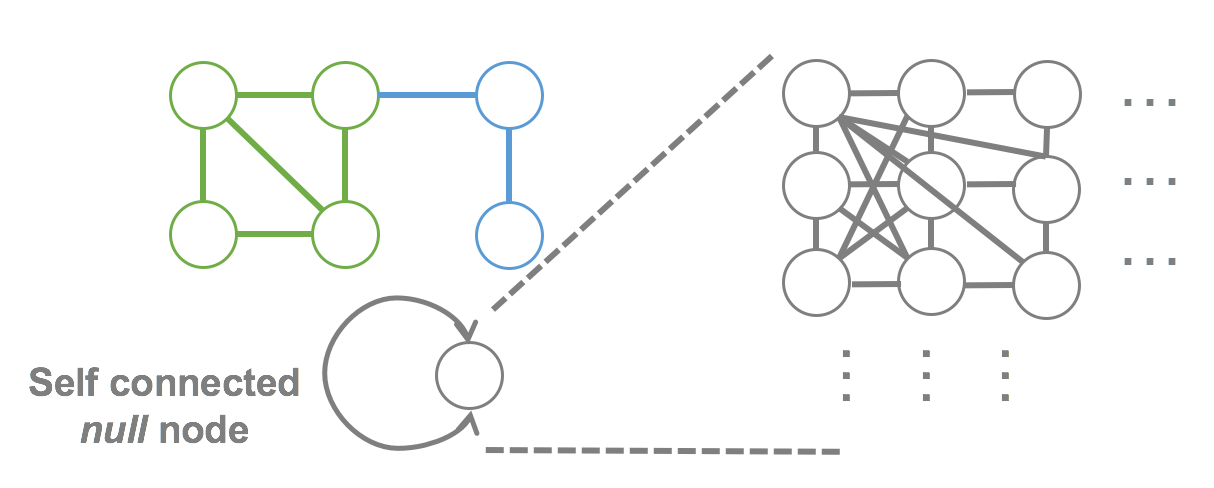
\includegraphics[width=0.46\textwidth]{figs/null_node_network.png}
	\caption[Caption for LOF]{\emph{The self linked/connected null node $\phi$ (grey) can be treated as a fully connected null node that can be matched to any pattern including background nodes. }}
	\label{fig:stochastic}
\end{figure}

After modified the compatibility function in the original algorithm, we are able to generate match result with both high recall and high precision. For instance, two graph with backgrounds nodes at the beginning and the end (in terms of their index) are not forced to match to each other (left) and end up match to the null node/the slack column/row in the end (right):
\begin{figure}[h]
	\centering
	\captionsetup{justification=centering}
	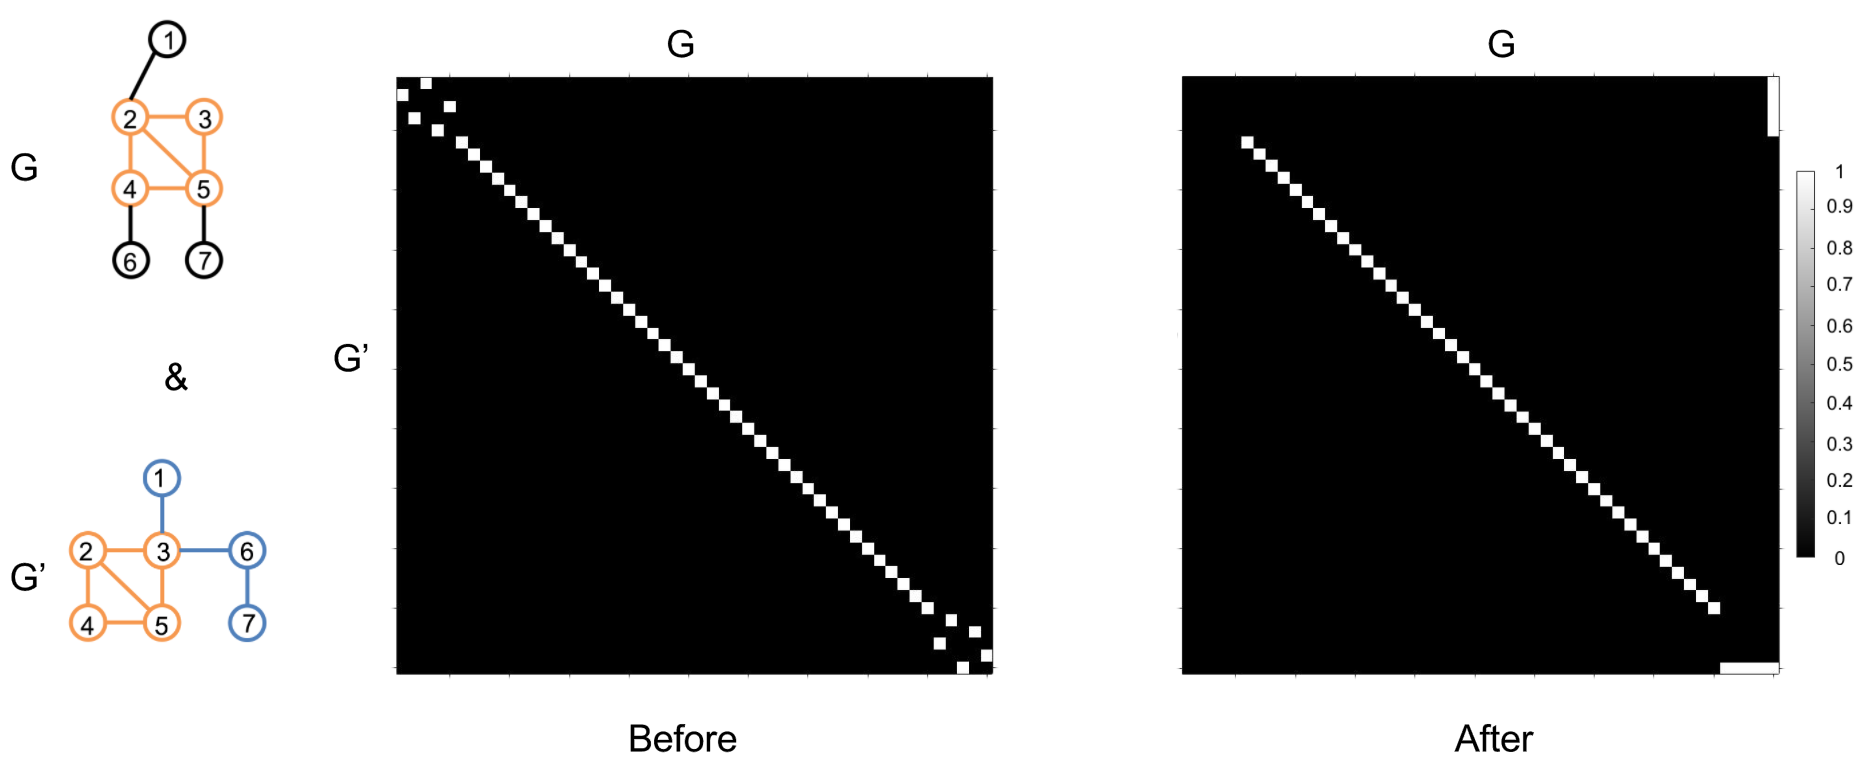
\includegraphics[width=0.8\textwidth]{figs/null_node_improve.png}
	\caption[Caption for LOF]{\emph{This is a visualization of the match matrixes produced by the original algorithm by Gold and Rangarajan (left) and the modified version (right).}}
	\label{fig:stochastic}
\end{figure}

\section{Conclusion}


In this chapter we introduced a graph matching algorithm that we improved and used to match the common sub-graph of two ARGs. If we do not apply the heuristic function, the match matrix $M$ shows us how likely one node in graph $G$ can be matched to another graph $G'$, which can in turn help us the summarize the common pattern among a set of graphs.



\chapter{Pattern Learning}

\section{Introduction}

Here in pattern learning, we extract the common pattern from a set of ARGs, and the extracted information can then be used to summarize the given ARGs and predict if a new ARG contains the common pattern we summarized. In our work, for instance, we can extract the common structure of a set of proteins that share the same function. The common structure we extracted can give us insight on how this structure can perform such function, and if a new protein also has the same structure that can carry out the same function.\\

To perform pattern learning, we utilize a probabilistic parametric model to represent the common pattern from the graphs (Hong\footnotemark and Huang 2004). Similar to how three normal distribution (or components) can capture the data distribution generated by $f(x)$ below, we used a couple component ARGs with various mean and variance to represent the common pattern:
\footnotetext{My dear advisor!}

\begin{figure}[h]
	\centering
	\captionsetup{justification=centering}
	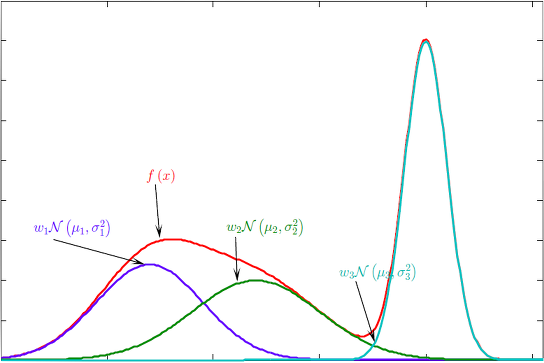
\includegraphics[width=0.65\textwidth]{figs/mixture.png}
	\caption[Caption for LOF]{\emph{The data distribution generated by $f(x)$ can be captured by three normal distribution with various means and variances.}}
	\label{fig:mixture}
\end{figure}

Therefore, the model training process is essentially training and setting up some component ARGs so that all the nodes and edges have the means and variances that best capture the common pattern in the given set of ARGs.\\

Based on the algorithm described by Hong and Huang, we first pick some ARGs from the input sample ARGs, and initialize them as the component ARGs. Then we perform an EM algorithm where on the \textbf{E}xpectation step we run the graph matching algorithm to calculate the matching probability between model ARGs and sample ARGs while on the \textbf{M}aximization step we update the model ARG (e.g. updating means, variances, and deleting redundant nodes) in order to achieve higher matching probability. Finally, once the update is very small, we output the model ARGs to represent the common pattern in sample ARGs:\\

\begin{figure}[h]
	\centering
	\captionsetup{justification=centering}
	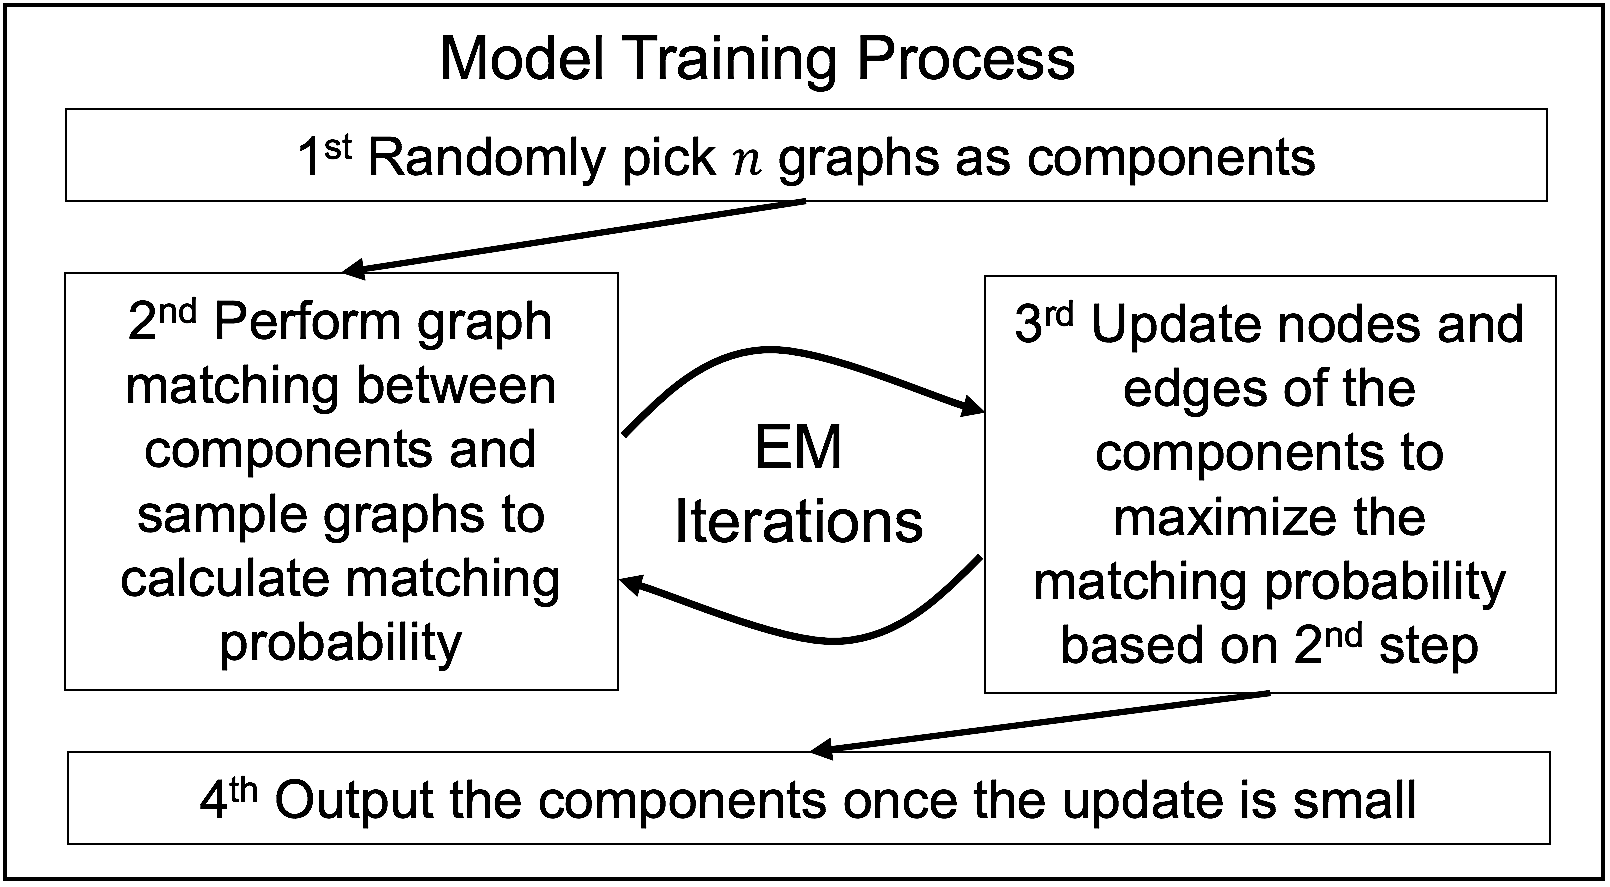
\includegraphics[width=0.8\textwidth]{figs/model_training.png}
	\caption[Caption for LOF]{\emph{The probabilistic parametric model training process with EM algorithm.}}
	\label{fig:model_training}
\end{figure}

\section{Syntax and Definition}

The sample ARGs (i.e. the set of ARGs we want to learn/extract pattern from) is denoted as $\{G_s\}_{s=1}^S$ where $S$ is the number of model components. Within each sample ARG, we indicate the label for each node and edge as $\overrightarrow{N^s_a}$ and $\overrightarrow{E^s_{ab}}$. This is similar to what we have in Chapter \ref{chap: graphmatching} but with an additional index $s$ indicating which sample $G$ these nodes and edges belong to. In addition, we denoted the real nodes in sample ARG, $G_s-\phi$, as $\widehat{G_s}$.\\

For the model, we denoted it as $Z$ and the model consists of a set of parametric model components $\{\Phi_w\}_{w=1}^W$ where $W$ is the number of model components. For each component, there are also an associated weight $\alpha_w$ which indicates how much information the component captures and how important the component is.\\

Within each component ARG, we indicate the mean for each node and edge as $\overrightarrow{N^w_a}$ and $\overrightarrow{E^w_{ab}}$ similar to what we have for sample ARGs, but with $w$ instead of $s$ indicating which model this node and edge belongs to. In addition to the mean, there are also the covariance matrixes for node and edge denoted by $\Sigma^w_a$ and $\Sigma^w_{ab}$ with a similar index. Last but not least, for each node in each component, there is an associated frequency/weight $\beta^w_a$ indicating how important one node is and if we can delete such node.\\

In addition, the matching algorithm introduced in Chapter \ref{chap: graphmatching} can generate match matrix $M^{sw}$ between sample ARG $G_s$ and component ARG $\Phi_w$ as well as the associated node/edge compatibility $C^{sw}$.

\section{Problem Definition}

Given a set of sample ARG $\{G_s\}_{s=1}^S$, our problem will be inferring the parameters in $Z$ including the number of components $W$, weight for each component $\alpha$, mean for each node/edge $\overrightarrow{N^w}$/$\overrightarrow{E^w}$, and the covariance associated with them $\Sigma$.\\

\begin{figure}[h]
	\centering
	\captionsetup{justification=centering}
	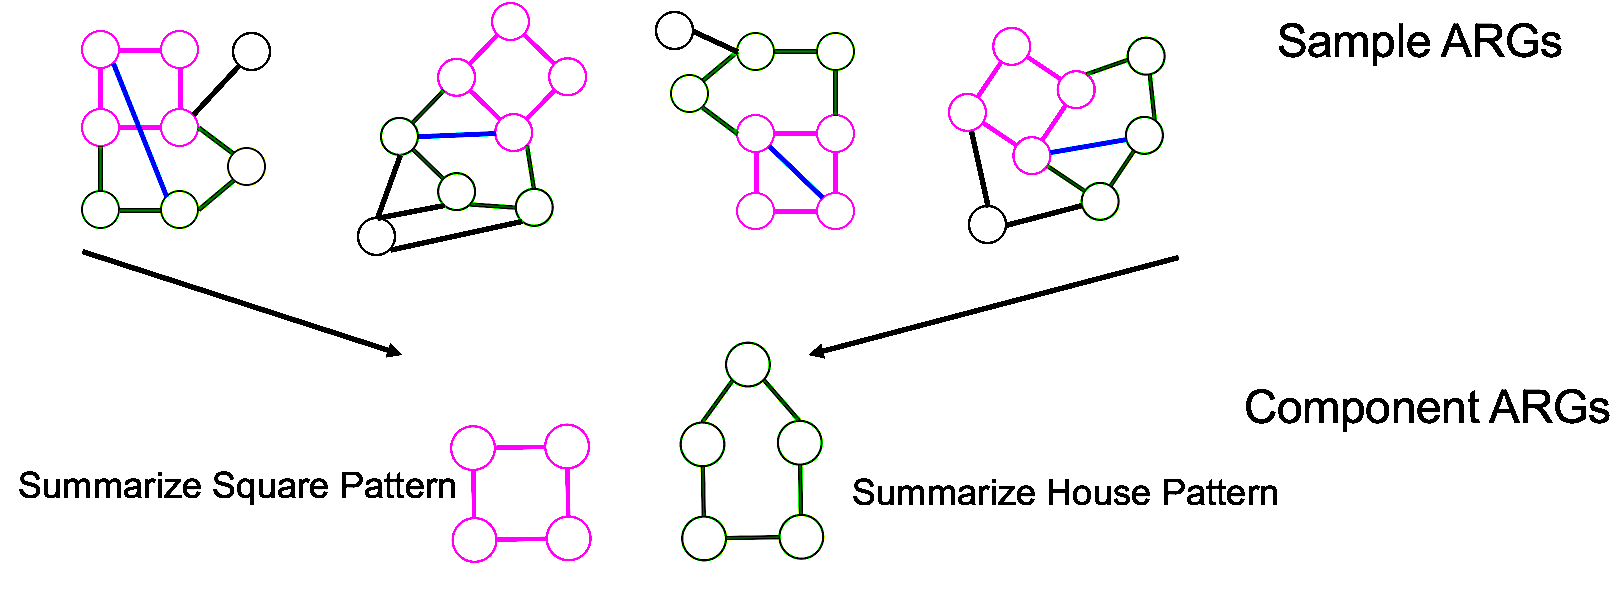
\includegraphics[width=0.8\textwidth]{figs/component_summary.png}
	\caption[Caption for LOF]{\emph{Component can summarize different part of the common pattern.}}
	\label{fig:component_summary}
\end{figure}

\section{Initializing the Components}

The first step of training the model is initializing the components in the model.\\

The way we do is manually pick $W$ random ARG from our sample set, and initialize them as component ARG $\Phi$. We took their original label as the mean, set their covariance matrix as the identity matrix $I$, and give equal weight to all the components and nodes. If we are converting a sample $G_s$ to a component $\Phi_w$, we would have:

\begin{align} 
\overrightarrow{N^w_a} & \leftarrow \overrightarrow{N^s_a} & \forall a \in \widehat{G_s}\\
\overrightarrow{E^w_{ab}} & \leftarrow \overrightarrow{E^s_{ab}}& \forall a,b \in \widehat{G_s}\\
\Sigma^w_a & \leftarrow  I\\
\Sigma^w_b  & \leftarrow  I\\
\alpha_w & \leftarrow \frac{1}{W}\\
\beta^w_a & \leftarrow \frac{1}{|G_s|}& \forall a \in G_s)
\end{align}\\

While we pick $W$ manually based on the complexity of the pattern here, theoretically, we can also start with a relatively larger number of components are delete some of them later. In terms of picking the sample, you can also do better than random by doing a pairwise graph matching among the sample ARG and choose ones that are the most representative based on the match matrixes $M$.

\newpage

\section{EM Algorithm}

Once we initialized the components $\{\Phi_w\}_{w=1}^W$ with all the parameters, we will then run through an EM algorithm to tune this parameters so our model $Z$ can capture the sample $\{G_s\}_{s=1}^S$ at its best. EM algorithm consist of an estimation step where we estimate how well our parameters perform and a maximization step where we tune the parameters to maximize the estimation. We run through these two steps iteratively until the tuning on the parameter is very small.

\subsection{Estimation Step}

In this step we estimate how well model $Z$ representing the sample ARG $G$ as $P(G|Z)$. Once we finish training the model, $f(G_{new}|Z)$ can also be used to predict if a new ARG $G_{new}$ contains the learned/extracted pattern. \\

The first thing we do in the estimation step is matching each component $\Phi_w$ with each sample $G_s$, and get a match matrix $M^{sw}$ from the graph matching algorithm introduced in Chapter \ref{chap: graphmatching}. In addition, the algorithm will also return the node and edge compatibility $C^{sw}$ computed as described in Section \ref{ssec:compatibility}.\\

Once we have the match matrix, we can calculate the probability of $G_s$ matching $\Phi_w$:

\begin{align} 
& \xi(G_s|\Phi_w)=\sum_{a=1}^{\widehat{G_s}}\sum_{i=1}^{\Phi_w}M^{sw}_{ai}C^{sw}_{ai}+ \sum_{a=1}^{\widehat{G_s}}\sum_{b=1}^{\widehat{G_s}}\sum_{i=1}^{\Phi_w}\sum_{j=1}^{\Phi_w}M^{sw}_{ai}M^{sw}_{bj}C^{sw}_{abij}\\
& P(G_s=\Phi_w)=\frac{\xi(G_s|\Phi_w)}{\sum_{t=1}^{W}\xi(G_s|\Phi_t)}
\end{align}\\

With $\xi(G_s|\Phi_w)$, we then can calculate:

\begin{equation} 
f(G|Z) = \sum_{w=1}^W\alpha_w\xi(G|\Phi_w) \label{eq:fgz}
\end{equation}\\

\subsection{Maximization Step}

In the maximization step, we adjust and tune the variable based on $P(G_s=\Phi_w)$, $M^{sw}$ and $C^{sw}$ that we calculated in the Estimation step.

\subsubsection{Update Component Weight}

First we update the component weight $\alpha_w$ for each component $\Phi_w$ as:

\begin{equation} 
\alpha_w=\frac{\sum^S_{s=1}P(G_s=\Phi_w)}{S}
\end{equation}\\

The component weight here is essentially calculating the average probability it matched to all the sample ARGs $\{G_s\}^S_{s=1}$.

\subsubsection{Update Component Node Frequency}

Then we update the frequency (i.e. weight) for each node in each component $\Phi_w$:

\begin{equation} 
\beta^w_a=\frac{\sum^S_{s=1}\sum^{\widehat{G_s}}_{i=1}M^{sw}_{ia}P(G_s=\Phi_w)}{\sum^S_{s=1}|\widehat{G_s}|P(G_s=\Phi_w)}
\end{equation}\\

The component node frequency is essentially an weighted average of the matching probability of this specific component node in all the matching matrix $M^{sw}$.\\

\subsubsection{Update Mean for Component Node}

To tune the mean for each component node, $\overrightarrow{N^w_a}$, we follow:

\begin{equation} 
\overrightarrow{N^w_a}=\frac{\sum^S_{s=1}\sum^{\widehat{G_s}}_{i=1}\overrightarrow{N^s_i}M^{sw}_{ia}P(G_s=\Phi_w)}{\sum^S_{s=1}\sum^{\widehat{G_s}}_{i=1}M^{sw}_{ia}P(G_s=\Phi_w)} \label{eq:nmean}
\end{equation}\\

Here we essentially calculated a weighted average of all the sample nodes, $\overrightarrow{N^s_i}$, based on how likely our component node matches to that sample node in match matrix $M^{sw}$ and how likely the component matches to that sample $P(G_s=\Phi_w)$.\\

\subsubsection{Update Covariance Matrix for Component Node}

Once we update the mean, we will also need to update the covariance matches $\Sigma^w_a$ for the component node:

\begin{equation} 
\Sigma^w_a=\frac{\sum^S_{s=1}\sum^{\widehat{G_s}}_{i=1}\overrightarrow{x^s_i}\overrightarrow{x^s_i}^TM^{sw}_{ia}P(G_s=\Phi_w)}{\sum^S_{s=1}\sum^{\widehat{G_s}}_{i=1}M^{sw}_{ia}P(G_s=\Phi_w)}
\end{equation}
where $\overrightarrow{x^s_i} = \overrightarrow{N^s_i} - \overrightarrow{N^w_a}$.\\

Similarly, here we essentially calculated a weighted average of covariance between the component node and sample nodes, $(\overrightarrow{N^s_i} - \overrightarrow{N^w_a})(\overrightarrow{N^s_i} - \overrightarrow{N^w_a})^T$, based on how likely our component node matches to that sample node in match matrix $M^{sw}$ and how likely the component matches to that sample $P(G_s=\Phi_w)$.\\

\subsubsection{Update Mean for Component Edge}

Similar to how we calculate the mean for component node $overrightarrow{N^w_a}$, we calculate the mean for component edge $\overrightarrow{E^w_{ab}}$ as:

\begin{equation} 
\overrightarrow{E^w_{ab}}=\frac{\sum^S_{s=1}\sum^{\widehat{G_s}}_{i=1}\sum^{\widehat{G_s}}_{j=1}\overrightarrow{E^s_{ij}}M^{sw}_{ia}M^{sw}_{bj}P(G_s=\Phi_w)}{\sum^S_{s=1}\sum^{\widehat{G_s}}_{i=1}\sum^{\widehat{G_s}}_{j=1}M^{sw}_{ia}M^{sw}_{bj}P(G_s=\Phi_w)}
\end{equation}

\subsubsection{Update Covariance Matrix for Component Edge}

Similar to how we calculate the covariance matrix for component node $\Sigma^w_a$, we calculate the covariance matrix for component edge $\Sigma^w_{ab}$ as:

\begin{equation} 
\Sigma^w_{ab}=\frac{\sum^S_{s=1}\sum^{\widehat{G_s}}_{i=1}\sum^{\widehat{G_s}}_{j=1}\overrightarrow{z^s_{ij}}\overrightarrow{z^s_{ij}}^TM^{sw}_{ia}M^{sw}_{bj}P(G_s=\Phi_w)}{\sum^S_{s=1}\sum^{\widehat{G_s}}_{i=1}\sum^{\widehat{G_s}}_{j=1}M^{sw}_{ia}M^{sw}_{bj}P(G_s=\Phi_w)}
\end{equation}
where $\overrightarrow{z^s_{ij}} = \overrightarrow{E^s_{ij}} - \overrightarrow{E^w_{ab}}$.\\

\subsubsection{Delete Redundant Node}

Since we initialized the component from sample ARGs, it is likely that the component itself will have background nodes (i.e. nodes not in the common pattern) that are redundant. To reduce the component ARGs from sample ARGs to the smaller common pattern, we can do node deletion based on the node frequency $\beta^w_a$ and some threshold. For instance, we choose to delete the $a$th node in $\Phi_w$ if:

\begin{equation} 
\beta^w_a < 1 - 0.85^n
\end{equation}
where $n$ indicate the $n$th round of the EM algorithm.\\

However, you can also choose to used a hard threshold like $0.85$ or delete redundant node in the very last round. In addition, we can also choose to delete redundant component here, even though we did not explore such option.

\subsubsection{Converge Condition and EM Algorithm Exit}

At the beginning of the EM algorithm, the maximization step will make large modification on each parameter, so we would go back to the estimation step after finishing the maximization step. \\

However, towards the end of the algorithm, we need to check if the EM algorithm has already converged (changes are small). If so, then we can exit the EM algorithm and go to the next step. Here, we simply compared previous component weight $\alpha^{(0)}$ with the current component weight $\alpha^{(1)}$, and exit if the differences is smaller than some number $\iota$:

\begin{equation} 
\sum^{W}_{w=1}\alpha^{(0)}_w<\iota
\end{equation}\\

However, this is not the only choices, and you can use other converging conditions if you like. Especially when your model only contains one component, you will have to use another condition since $\alpha_w$ will always be $1$.\\

\newpage

\section{Detect the Spatial Pattern}

Once we finished training the model, how do we detect or predict if the extracted/summarized pattern exist in a new ARG? As mentioned above, we can use $f(G|Z)$ calculated by Eq.\ref{eq:fgz} as our similarity score to determine if the new ARG, $G$, contains the same spatial pattern as the training samples. Therefore, we would need to setup some sort of threshold, $\chi$, so that $G$ contains the learned pattern only if $f(G|Z)>\chi$.\\ 

To setup $\chi$, we generate a set of $R$ random graphs $\{G^r\}^{R}_{r=1}$ with similar number of nodes, edge connectivity\footnotemark, and labels as our training sample $\{G^s\}^{S}_{s=1}$. With the random generated ARGs, we can calculate a set of similarity score $\{f(G^r|Z)\}^{R}_{r=1}$ that can help us determine the threshold $\chi$. If you have enough computational power, and are able calculate the similarity score for a very large number\footnotemark of random ARG. You can simply take the $99.99\%$ percentile of the similarity score set $\{f(G^r|Z)\}^{R}_{r=1}$.\\
\footnotetext{How many nodes one node connected to.} 

However, unlike Google\footnotemark, we do not live in a magic land. Therefore, we only calculated the similarity score for $50$ random ARGs and run z-test on the set of similarity scores $S=\{f(G^r|Z)\}^{R}_{r=1}$ which allows us to set the threshold $\chi$ as $\chi \leftarrow \mu+3\sigma$ where $\mu$ and $\sigma$ are the mean and variance of the similarity scores of random ARGs.
\footnotetext{Let's say $R>1,000,000$.}
\footnotetext{https://twitter.com/deliprao/status/842635509255962624}\\

Due to the application of our model, we do not consider the case where a random but much larger graph could potentially score a higher similarity simply because there are more node to sum. Therefore, if your application are dealing with ARGs on a large spectrum of node number, you might need to modify $f(G|Z)$ to factor in $|G|$.

\section{Implementation Detail}

\subsection{Coding Complexity}

While the model introduced here seems to be pretty straight forward, the actual coding is rather tedious since we have many steps, parameters and nested summation. Therefore, we break down the algorithm and modulated each step so it is easier to debug.

\subsection{Null Node in the Model}

While it is not mentioned above, the model we implemented actually has a null node $\phi$, but it does not have any label on the node or edges. Instead, the graph matching algorithm will ignore this null node and used its own null node definition as described in Section \ref{ssec:nullnode}. However, when the graph matching return the match matrix and compatibility, $M^{sw}$ and $C^{sw}$, they include the value for algorithm's own null node which we can used for the model null node. Such implementation allows us to use the graph matching algorithm developed earlier with very little modification and save the troubles of maintaining the parameters for the null node.

\subsection{Run Time}

We trained a model with $2$ components on $5$ pattern embedded ARG with $\sim30$ nodes, and it took $\sim 30$ minutes including the time for setting up the pattern detection threshold $\chi$. As mentioned in Section \ref{ssec:graphmatchingruntime}, you can adjust the parameter for converging condition and learning rate to tradeoff between accuracy and running time.

\section{Testing the Model}

Similar to how we generated test cases in Section \ref{sec:graphmatchingtest} for graph matching algorithm, we generate a set of ARGs with ($G^p$) or without ($G^r$ i.e. random ARG) the embedding pattern. \\

Then we train a model on some of the ARGs with the pattern (i.e. $G^p$) and plot a histogram of the similarity score ($f(G|Z)$) for all $G^p$ and $G^r$. This is a sample result generated by a set of ARGs with $\sim30$ nodes, and the model is trained by $5$ sample ARGs with $2$ component ARGs.:

\begin{figure}[h]
	\centering
	\captionsetup{justification=centering}
	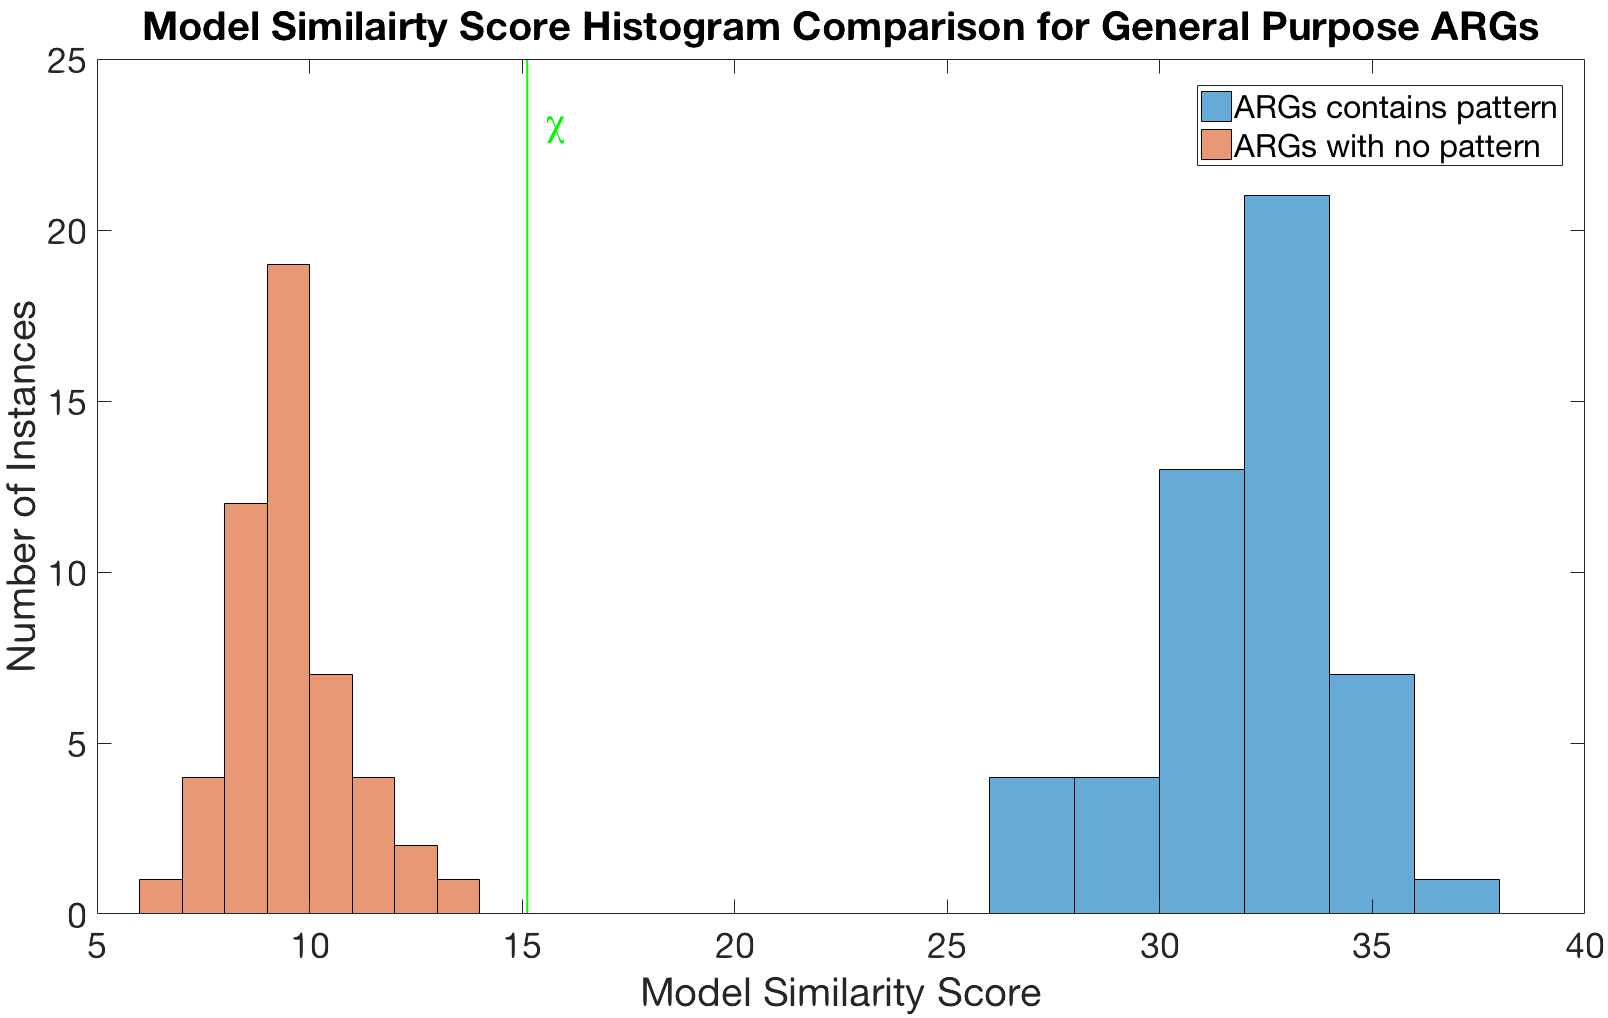
\includegraphics[width=0.9\textwidth]{figs/pattern_learning.png}
	\caption[Caption for LOF]{\emph{Similarity Score $f(G|Z)$ for pattern embedded ARG (blue) and random ARG(orange) while the green vertical line is the threshold $\chi$.}}
	\label{fig:pattern_learning}
\end{figure}

\section{Conclusion}

In this chapter we introduced a probabilistic parametric model $Z$ that we can train via EM algorithm. This model allows us to learn the common/share pattern among a set of ARGs, and used a set of component ARGs to represent/summarize such pattern. By calculating $f(G|Z)$ and comparing it to the threshold $\chi$, we can predict if a new ARG $G$ contains the learned pattern.\\

If we can model a protein crystal structure as an ARG, we can potentially use this model to mine novel protein structure or functional structure from protein crystallography data.









\chapter{Protein Modeling}

\section{Introduction}

\chapter{Looking Forward}

\section{Graph Matching}

\subsection{More Efficient Implementation}

While the graph matching algorithm is already an approximation, it is still not fast enough to support the pattern learning model to learn in very large scale. Therefore, a more efficient implementation is of interest from an engineering view point and if we want to move the algorithm to production system.\\

One major time sink of the algorithm is the iterative row and column normalizations enforcing by the two-way constraints. A potential solution would be using GPU to perform row/column normalization independently in parallel fashion. Another solution would be ignoring the normalizations altogether, and incorporating the two-way constraints into our objective functions with Lagrange multipliers:

\begin{align}
E(M)=&-\frac{1}{2}\sum_{a=1}^{G}\sum_{i=1}^{G'}\sum_{b=1}^{G}\sum_{j=1}^{G'}M_{ai}M_{bj}C_{abij}\nonumber\\
&-\frac{1}{\beta}\sum_{a=1}^{G}\sum_{i=1}^{G'}M_{ai}(\text{log}M_{ai}-1)\nonumber\\
&+\sum_{a=1}^{G}\mu_a(\sum_{i=1}^{G'}M_{ai}-1)+\sum_{i=1}^{G'}\nu_a(\sum_{a=1}^{G}M_{ai}-1)
\end{align}

and we can directly derive $M$ via the objective function using library like Theano\footnotemark. However, because of the nested sum, even though there is a matrix operation that can help us do the forward calculation, the back-propagation/derivation has not been implemented yet. Therefore, we did not implement such solution, but it would be much more efficient once the derivation for such operations are implemented.\\
\footnotetext{http://www.deeplearning.net/software/theano/}

Another time and memory sink for the algorithm would be the compatibility between edges. While the computation can be speed up via parallel computing, there are lots of communication overhead due to the design of the edge compatibility matrix, where each row or column is associated with a single edge in the graph and result in a $(|G|*|G|)\times(|G'|*|G'|)$ matrix. Since MATLAB only allows parallel computing row by row or column by column, we are still copying a huge vector in parallel task which result in lots of communication overhead. In addition, the compatibility matrix is very huge and could result in memory issue. Even though we can fix by storing it as a sparse matrix, sparse matrix could also introduce lots of computation overhead during the graduated assignment process.\\

Therefore, it would be beneficial for us to think of another representation for edge compatibility scores that are both memory and computation efficient.

\subsection{Automate Parameters Tuning}

A lot of the frustrations during the development of this algorithm coming from tuning the parameter considering the large number of different combinations of parameter. Considering different application of the same algorithm could have very different optimal parameters configuration, it would be beneficial for users if the algorithm has some mechanisms to tune the parameter automatically based on the expected matching result.\\

While this problem can easily turn into another project about model learning, we can start from a simple grid search, or learn about how different parameters could affect different aspects of the matching result and adjust them accordingly.


\section{Pattern Learning}

\subsection{Smarter Component Initiation}

In our model, the initial components can have a huge impact on model's pattern learning quality. For instance, if the share pattern has two components but our starting components only have one of them, the model could never capture the entire pattern. Therefore, we might want to be smarter than random when initializing our model components.\\

One potential solution would be do a pairwise graph matching before picking the components, and incorporate some heuristic rules (e.g. matching result clarity, larger matching nodes etc) to help us pick the components.\\

Another solution would be introducing a mechanism allows the model to swap in random sample ARGs as new components, and switch it our if the performance does not get better.

\subsection{Component and Node Deletion}

Since we start off with sample ARGs as our components ARGs, it is important for the components ARGs to reduce themselves in order to accurately represent the share pattern. However, in many of our experiments, the node deletion is not always perfect just based on a threshold. Therefore, we might want to introduce more heuristic rules for deletion in the future. One such rule could be examining $\beta^w$ across multiple rounds, and only delete it based on a history of pattern.\\

In addition to node deletion, it would be helpful if we could delete the entire component as well since the randomly initialized components could share similar pattern, and therefore become redundant. Introducing a mechanism for component deletion not only allow us to start from a relatively large pool of components, but also help us speed up the model training. One potential way we could do this is by comparing the result of two components matching to the same sample ARG.

\subsection{Other Applications}

Besides protein structure mining, another interesting application for the pattern learning model would be computer vision, which is dominated by Neural Network nowadays.\\

Neural Network like CNN(Convolutional Neural Network) is a very effective model for object recognition because the non-linear transformation and back-propagation are able to learn features automatically and effectively. Moreover, pooling layer has been effective in handling minor variance while different filters can handle large variance like rotation\footnotemark. However, when the scene becomes more complicated, describing the relationship between multiple object for instance, CNN becomes less effective (larger model and more training data) because CNN is more effective in learning features, but less effective in modeling relationship. For instance, if we have two objects whose relationship is a certain distance (A), to recognize the same relationship after rotation (B), a CNN might need to learn an additional filter for the $45^\circ$ angle, while an ARG representation can easily recognize the rotated scene with no trouble:\\
\footnotetext{Filters might not be representing different rotations exactly but rotation certainly requires more filters to summarize more features.} 

\begin{figure}[h]
	\centering
	\captionsetup{justification=centering}
	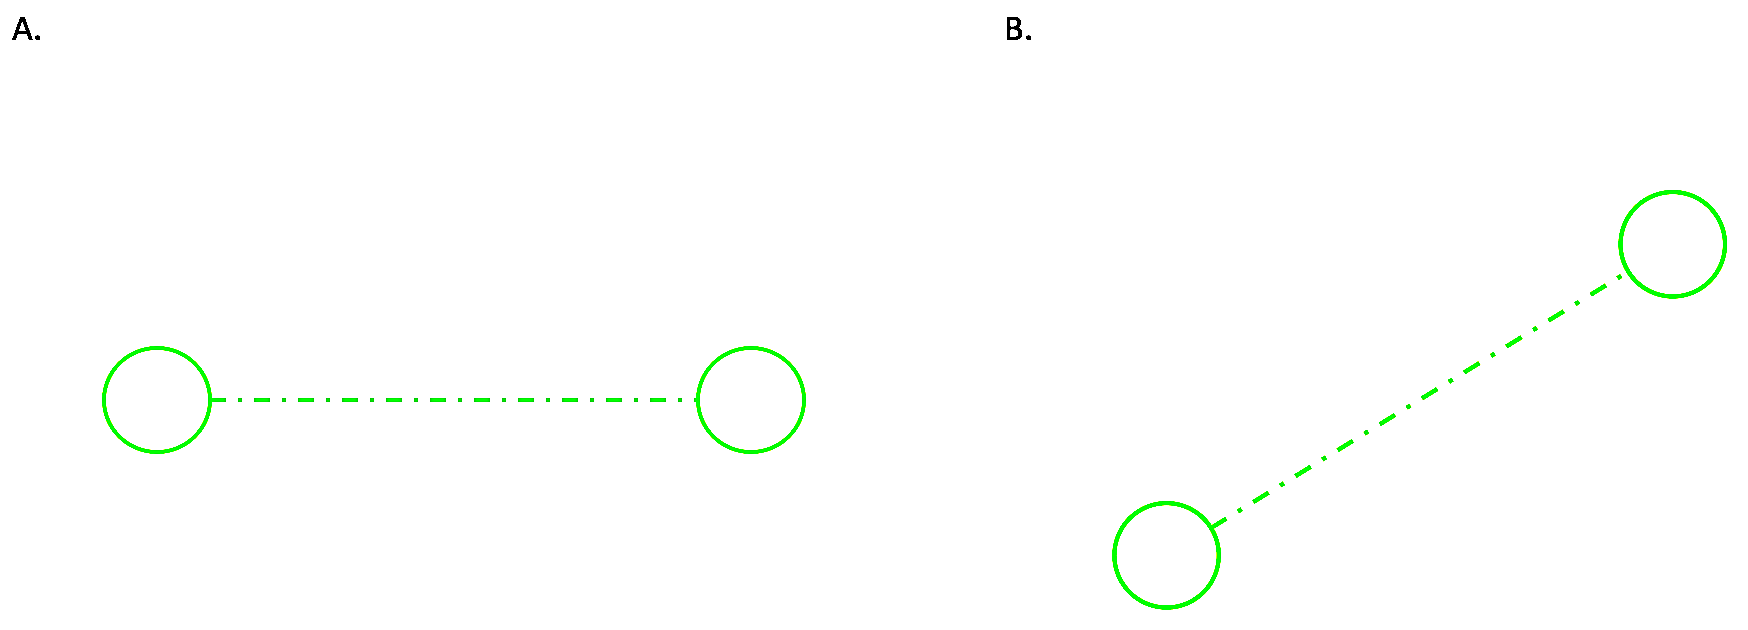
\includegraphics[width=0.8\textwidth]{figs/rotation.png}
	\caption[Caption for LOF]{\emph{A. Two objects (circles) have a relationship of a certain distance $X$.\\ B. A rotated scene showing such relationship. }}
	\label{fig:rotation}
\end{figure}

Therefore, the pattern learning model described here can be very helpful in understanding the relationship between complex scene ("student taking class", "cars stuck in traffic" etc.) while CNN helps the model to recognize individual object in the scene or generate latent representation for individual object.\\

Besides computer vision, the pattern learning model can also be used in natural language processing task, like modeling the relationship (e.g. Q\&A, extension, agreement, etc.) between sentences in a dialogues. Here, we can turn each word/concept to a node (whose label can be the word vector) and the word/concept distance as the edge. Once we turn the conversation exchange into an ARG, we might be able to model different relationship as well.\\

Therefore, combining neural network for individual object and pattern learning for modeling relationship, machines probably can learn complex structure, scenes, conversations and many other things more effectively. I am really excited about what's coming next.

\section{Protein Modeling}

\subsection{Novel Structure Motif in Protein}

While the proof of concept we did in Section \ref{sec:poc} is nice, domain discovery is not a very challenging task. Due to its relatively large size, simple 3D alignment should give you a reasonably good match and you don't really need to model the protein as an ARG.\\

However, if we are able to train the model efficiently with enough data, we might be able to discover 3D structure motifs that have long been overlooked by sequential matching algorithm. If the model can learn such novel motif, it would be of great help for many biologists.

\subsection{Protein as Documents and Amino Acid as Word}

In Section \ref{sssec:a2v}, we treated protein as documents and amino acid as word, which allows us to use model in natural language field to generate representation for amino acid.\\

In the same line, many of the models developed today in the natural language field, especially the kinds dealing with sequential model, might be a great tool for answering question about protein. For instance, we can use a Seq2Seq model to predict structure of protein sequence, or use LSTM model to predict protein chemical property with the protein sequence.


\subsection{Edge for Protein ARG Revisit}

While tuning hyper parameters for the model, we realized that the node compatibility needs to play a more important role(larger $\alpha$) in order to get clear and correct result for graph matching. This makes sense because protein alignment should be driven more by the amino acid compatibility. However, can we give edge here a different representation and a more effective relationship to help with matching/alignment?



\chapter*{Appendix}

Here are the code and presentation for the thesis.\\

Graph Matching Implementation Code and Documentation:

https://github.com/WesleyyC/Graph-Matching\\

Pattern Learning Implementation Code and Documentation:

https://github.com/WesleyyC/Spatial-Pattern-Learning\\

Protein Modeling Implementation Code and Documentation:

https://github.com/WesleyyC/Proteins-Domain-Learning\\

Thesis Presentation:

https://github.com/WesleyyC/Senior-Thesis/blob/master/Senior\_Thesis\_Presentation.pdf

% ------------ Bibliography ----------------

\nocite{*}
\printbibliography

% ------------ Appendices ----------------

\end{document}

\end{document}
